\chapter{Introdução}
\label{cap:introducao}

Cada vez mais à tecnologia avança numa velocidade impressionante. Com esse avanço se tornou possível ter computadores com um enorme poder de processamento à um menor custo e ocupando menos espaço. Com isso, algoritmos complexos de inteligência artificial realizam seus cálculos muito mais rápido, além de que, com o tempo, eles foram se tornando cada vez mais robusto. \cite{rodrigues2017fundamentos} 

A inteligência artificial (IA) vem evoluindo muito desde à criação do seu conceito, em 1956. Inicialmente, IA era utilizada apenas para à resolução de problemas simples e repetitivos, com aplicação de regras lógicas. Porém, com a chegada da Aprendizagem Profunda (\textit{Deep Learning}) os algoritmos passaram a poder realizar tarefas mais complexas como reconhecimento de fala e classificação de imagens. \cite{goodfellow2016deep}

Com o avanço da eletrônica e dos \textit{hardwares} tornou-se possível desenvolver veículos que possuem sistemas embarcados e realizam tarefas de forma totalmente independente, ou seja, autônoma. \cite{rodrigues2017fundamentos}

No brasil, à indústria automobilística representa 18,2\% da economia nacional, segundo dados de 2011. À adoção de padrões de qualidade, o aumento do nível de exigência dos consumidores e à concorrência do mercado são fatores que impactam diretamente na necessidade de inovação dos veículos produzidos, estimulando o investimento em novas tendências tecnológicas. Entre todas essas tendências, é possível afirmar que à condução autônoma é a mais revolucionária da atualidade. Ela mudará toda à concepção de locomoção veicular que temos. \cite{ rodrigues2017fundamentos}

Os carros autônomos trarão diversos benefícios para sociedade. Uma redução na taxa de acidentes e até no engarrafamento será algo notório quando essa revolução acontecer. Já para os motoristas, um dos maiores atrativos é a possibilidade de realizar outras tarefas enquanto o carro dirige, além de ter uma notória economia de combustível já que ele é controlado por um computador e realiza aceleração e frenagem de forma bem mais preciso que um ser humano. Todos esses fatores se mostraram bastante atraentes para as grandes empresas automobilísticas que entraram com tudo na corrida de desenvolvimento de carros autônomos. \cite{inproceedings,rodrigues2017fundamentos}

Apesar das diversas vantagens dos veículos autônomos, eles ainda terão diversos desafios para entrar no mercado. Dentre eles, as responsabilidades legais sobre os eventos consequentes de suas ações, na qual o veículo não pode ser responsável por possíveis acidentes causados por ele. Para isso, o motorista deve ser responsável por qualquer coisa que venha acontecer e tenha à possibilidade também de monitorar e tomar o controle do veiculo caso seja necessário. \cite{inproceedings}

Outro problema para os veículos autônomos é a legislação de trânsito. Atualmente ela não permite à circulação desses veículos no Brasil. É necessário que haja acréscimo de leis de acordo com as necessidades técnicas e administrativas de cada estado e município.\cite{inproceedings}

Devido à necessidade de sensores, atuadores, dispositivos computacionais e manutenção, os preços dos veículos autônomos são bem mais elevados se comparado aos veículos não autônomos. \cite{inproceedings}

\section{Motivação}
\label{sec:motivacao}

Segundo Elon Musk, CEO da \textit{Tesla Motors}, em 2020 já teremos carros autônomos em circulação\cite{elonmusk}, porém o Brasil se encontra em 17º no rank divulgado pelo G1\cite{brasilutimorank} de países mais aptos à receber à tecnologia, apesar de ter uma excelente aceitação pelos brasileiros, até maior que japoneses. 

As pesquisas divulgadas pelo G1 mostram o quão grande é à dificuldade de aplicação de tecnologia no Brasil. Segundo o rank divulgado pela KPMG, o país ocupa à última posição no rank de política e legislação e o penúltimo no rank de infraestrutura. Isso mostra que, apesar do país ter bastante dificuldades governamentais para a aplicação e desenvolvimento do projeto, não faltam pessoas querendo adquirir essa tecnologia e à corrida para o desenvolvimento desses veículos no país já começou. 

Projetos como o Smart Camaro, IARA, caRINA, e Wally, mostrados na figura \ref{carrosautonomos} \cite{carroautonomobrasil} já estão em desenvolvimento nas universidades do pais, porém é necessário conhecimentos profundos em ROS (\textit{Robot Operating System}), programação em C++ e Python, fusão de sensores, visão computacional, programação em GPU (\textit{Graphics Processing Unit}), além de entendimento sobre \textit{hardware}.

	\begin{figure}[H]
		\centering
		\Caption{\label{carrosautonomos} Smart Camaro, IARA, caRINA, e Wally em ordem}
		\UNIFORfig{}{
			\fbox{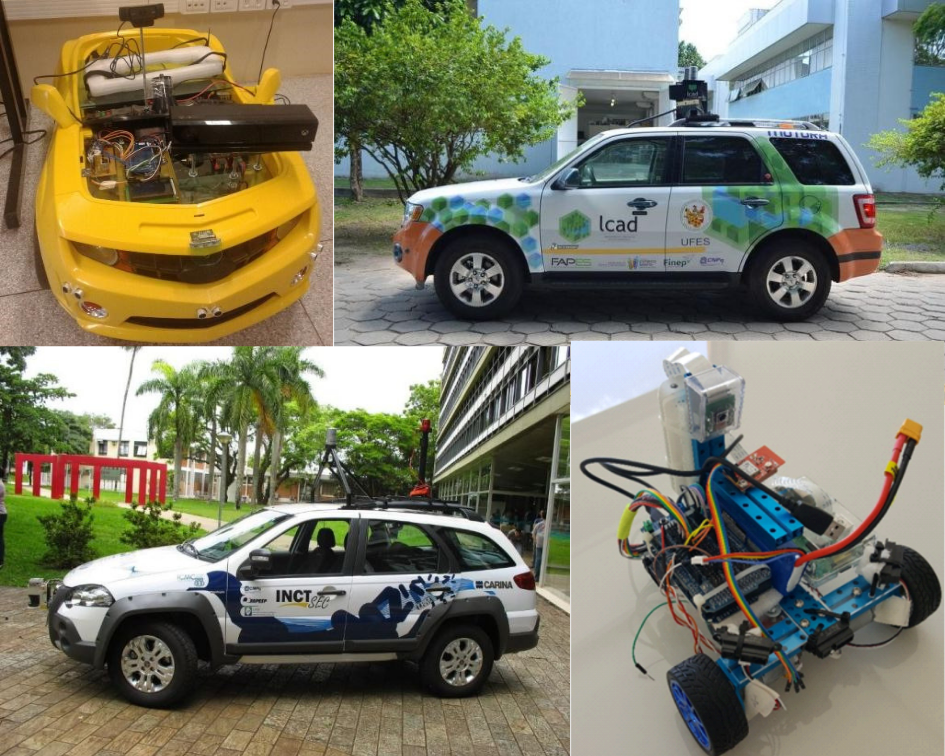
\includegraphics[width=16cm]{fig/carrosAutonomo.png}}
		}{
			\Fonte{\cite{carroautonomobrasil}}
		}	
\end{figure}

\section{Objetivos}
\label{sec:objetivos}

\subsection{Objetivo Geral}
\label{sec:objetivo-geral}

Adaptar o algoritmo do projeto \textit{Car Behavioral Cloning} para Plataforma Robótica Jaguar utilizando apenas uma câmera e utilizar imagens capturadas por ela para treinar o algoritmo de inteligencia artificial e fazer com que o Jaguar pilote de forma autônoma.


\subsection{Objetivos Específicos}
\label{sec:objetivos-especificos}

\begin{enumerate}
\item Instalar o ROS \textit{Kinetic} no Ubuntu de Versão 16.04 LTS, criar o \textit{Workspace} e instalar todos os pacotes;
\item Instalação do Python 3.5.2 e bibliotecas para ambas as versões do Python 2.7 e 3.5.2;
\item Alterar as configurações de rede do computador para conectar à máquina com o Jaguar;
\item Obter as imagens e comandos de direção e velocidade do treino nas pistas;
\item Pilotar o Jaguar em pelo menos duas pistas em diferentes direções;
\item Treinar o algoritmo para o controle autônomo da Plataforma Robótica Jaguar com diferentes parâmetros;
\item Testar os modelos criados nas pistas utilizadas para o treinamento;
\item Avaliar o desempenho do Jaguar nas diferentes pistas, em diferentes direções e com diferentes padrões de treinamento e tirar uma conclusão dos resultados;
\end{enumerate}